\documentclass{uni_tue_template}

\usepackage{color}
\usepackage[colorlinks]{hyperref}
\definecolor{darkred}{rgb}{0.5,0,0}
\definecolor{darkgreen}{rgb}{0,0.5,0}
\definecolor{darkblue}{rgb}{0,0,0.7}
\hypersetup{
			linkcolor={darkblue},
			filecolor={darkgreen},
			urlcolor={darkred},
			citecolor={darkblue},
}

\usepackage[export]{adjustbox}
\usepackage{tikz}
\usetikzlibrary{shapes}
\usepackage{rotating}
\usepackage{sistyle}

\lstdefinestyle{sql}{%
	language=SQL,%
	commentstyle=\color{comment},%
	stringstyle=\color{string},%
	keywordstyle=\color{keyword}\bfseries,%
	morekeywords={text, real, begin},%
	basicstyle=\ttfamily\footnotesize,%
	numbers=left,
	numberstyle=\tiny\color{black},
	stepnumber=1,
	showstringspaces=true,%
	columns=fixed,%
	moredelim=[is][\itshape]{@@}{@@},%
	tabsize=2
}
\lstset{aboveskip=-.05cm,style=sql, firstline=4}

\newcommand{\otext}[1]{\overset{\mathclap{\rule[-.3\baselineskip]{0pt}{0cm}\textmd{#1}}}}
\newcommand{\set}[1]{\mathbb{#1}}
\newcommand{\code}[1]{\texttt{{\footnotesize #1}}}
\newcommand{\md}[1]{\textmd{#1}}

% content of left head area e.g. subject like ETI
\def \headLeft{Andreas Schmied (3087156),\newline Tobias Stumpp (3798377)}

% content of center head area, used for names
\def \names{\"Ubungsblatt 6,\\ Datenbanksysteme II}

% content of right head area e.g. semester like WiSe 2012/13
\def \headRight{\today}

% set name for exercises
\def \exerciseName{Aufgabe}

\begin{document}
\exercise{}\\
\emph{Stellen Sie sich vor, eine Datenbankseite kann höchstens vier Werte vom Typ \code{INTEGER} enthalten. Konstruieren Sie B\textsuperscript{+}-Bäume der Ordnung $d=2$, so dass sich folgende Szenarien einstellen:}
\subExBegin{1{.}}
  \item \emph{Einen B\textsuperscript{+}-Baum, in welchem das Löschen des Schlüssels 25 zu einer Umverteilung (\emph{redistribution}) auf Blattebene führt. Zeigen Sie die Struktur des Baumes vor und nach dem Entfernen des Schlüssels.}\\
  \begin{tabular}{cc}
    vor Entfernen & nach Entfernen\\
    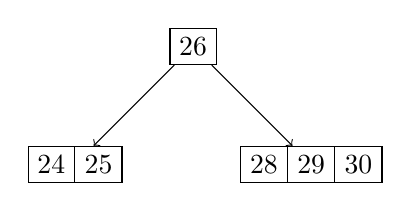
\begin{tikzpicture}
      \tikzstyle{bplus}=[rectangle split, rectangle split horizontal,rectangle split ignore empty parts,draw]
      \tikzstyle{every node}=[bplus]
      \tikzstyle{level 1}=[sibling distance=30mm]
      \tikzstyle{level 2}=[sibling distance=15mm]
      \node {26} [->]
        child {node {24 \nodepart{two} 25}}
        child {node {28 \nodepart{two} 29 \nodepart{three} 30}}
    ;\end{tikzpicture}
    &
    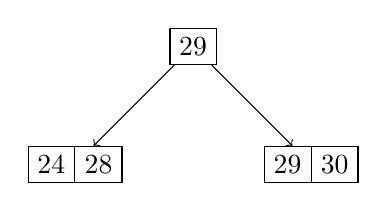
\begin{tikzpicture}
      \tikzstyle{bplus}=[rectangle split, rectangle split horizontal,rectangle split ignore empty parts,draw]
      \tikzstyle{every node}=[bplus]
      \tikzstyle{level 1}=[sibling distance=30mm]
      \tikzstyle{level 2}=[sibling distance=15mm]
      \node {29} [->]
        child {node {24 \nodepart{two} 28}}
        child {node {29 \nodepart{two} 30}}
    ;\end{tikzpicture}
  \end{tabular}
  \item \emph{Einen B\textsuperscript{+}-Baum, in welchem das Löschen des Schlüssels 25 zu einer Verschmelzung (\emph{merge}) von zwei Knoten auf Blattebene führt, aber ohne die Höhe des Baumes zu ändern.}\\
  \begin{tabular}{cc}
    vor Entfernen & nach Entfernen\\
    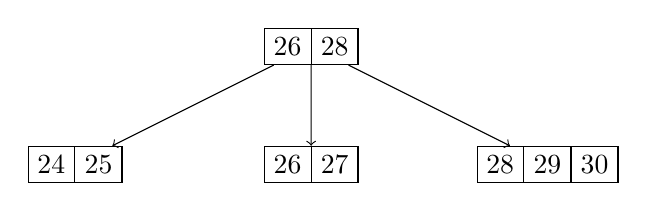
\begin{tikzpicture}
      \tikzstyle{bplus}=[rectangle split, rectangle split horizontal,rectangle split ignore empty parts,draw]
      \tikzstyle{every node}=[bplus]
      \tikzstyle{level 1}=[sibling distance=30mm]
      \tikzstyle{level 2}=[sibling distance=15mm]
      \node {26 \nodepart{two} 28} [->]
        child {node {24 \nodepart{two} 25}}
        child {node {26 \nodepart{two} 27}}
        child {node {28 \nodepart{two} 29 \nodepart{three} 30}}
    ;\end{tikzpicture}
    &
    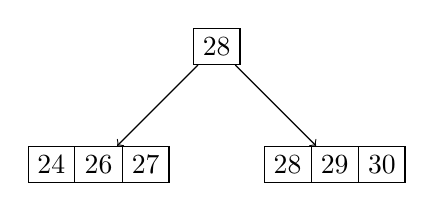
\begin{tikzpicture}
      \tikzstyle{bplus}=[rectangle split, rectangle split horizontal,rectangle split ignore empty parts,draw]
      \tikzstyle{every node}=[bplus]
      \tikzstyle{level 1}=[sibling distance=30mm]
      \tikzstyle{level 2}=[sibling distance=15mm]
      \node {28} [->]
        child {node {24 \nodepart{two} 26 \nodepart{three} 27}}
        child {node {28 \nodepart{two} 29 \nodepart{three} 30}}
    ;\end{tikzpicture}
  \end{tabular}
\subExEnd{}
%
\newpage 
%
\exercise{}
\subExBegin{1{.}}
  \item \emph{Betrachten Sie für diese Aufgabe zunächst den k-d Baum in Abbildung 1. Auf welche Schlüsselwerte (Knoten und Blätter) der Baumes muss zugegriffen werden, um die folgenden Queries zu beantworten?}
  \begin{enumerate}[{(}a{)}]
    \item \emph{\code{salary = 120}}\\
    \vspace*{-1.3cm}\\
    \[(140,85), (100,50), (60,40), (110,70), (120,50)\]
    \vspace*{-1.3cm}\\
    \item \emph{\code{age = 50}}\\
    \vspace*{-1.3cm}\\
    \[(140,85), (100,50), (110,70), (75,45), (120,50), (350,45), (275,50),
    (270,60)\]
    \vspace*{-1.3cm}\\
    \item \emph{\code{salary <= 300 AND age <= 40}}\\
    \vspace*{-1.3cm}\\
    \[(140,85), (100,50), (60,40), (60,25), (350,45), (400,25), (260,30)\]
     \vspace*{-1.3cm}\\
  \end{enumerate}
  \item \emph{Eine alternative Strategie um mehrere Attribute in einem Schlüssel zusammenzufassen sind B\textsuperscript{+}-Bäume mit \emph{composite search-keys}. Konstruieren Sie einen B\textsuperscript{+}-Baum mit einem solchen zusammengesetzten Schlüssel \code{<salary,age>} und $d=2$ aus den Schlüsselwerten des k-d Baumes in Abbildung 1. Sortieren Sie dazu die Tupel entsprechend und bauen Sie den Baum mit Hilfe der \emph{bulk loading} Methode auf.}\\
  Der \emph{composite search-key} entspricht der Verknüpfung der 10-Bit langen Binärdarstellungen von \code{salary} und \code{age}:\\
  \vspace*{-.7cm}\\
  \[\begin{array}{|c|c|c|c|}
  \hline
  $<salary, age>$ & \multicolumn{3}{c|}{$Verknüpfung$}\\
  & \multicolumn{2}{c|}{$binär$} & $dezimal$\\
  \hline
   (60,25) & 0000\;1111\;00 & 00\;0001\;1001 &  61465\\
   (60,40) & 0000\;1111\;00 & 00\;0010\;1000 &  61480\\
   (75,45) & 0001\;0010\;11 & 00\;0010\;1101 &  76845\\
  (100,50) & 0001\;1001\;00 & 00\;0011\;0010 & 102450\\
  (110,70) & 0001\;1011\;10 & 00\;0100\;0110 & 112710\\
  (120,50) & 0001\;1110\;00 & 00\;0011\;0010 & 122930\\
  (140,85) & 0010\;0011\;00 & 00\;0101\;0101 & 143445\\
  (260,30) & 0100\;0001\;00 & 00\;0001\;1110 & 266270\\
  (270,60) & 0100\;0011\;10 & 00\;0011\;1100 & 276540\\
  (275,50) & 0100\;0100\;11 & 00\;0011\;0010 & 281650\\
  (350,45) & 0101\;0111\;10 & 00\;0010\;1101 & 358445\\
  (400,25) & 0110\;0100\;00 & 00\;0001\;1001 & 409625\\
  (500,35) & 0111\;1101\;00 & 00\;0010\;0011 & 512035\\
  \hline
  \end{array}\]
  Mit \code{bulk loading} aufgebauter B\textsuperscript{+}-Baum:\\
  \vspace*{-1.4cm}\\
  \begin{center}
  \begin{sideways}
  \begin{small}
  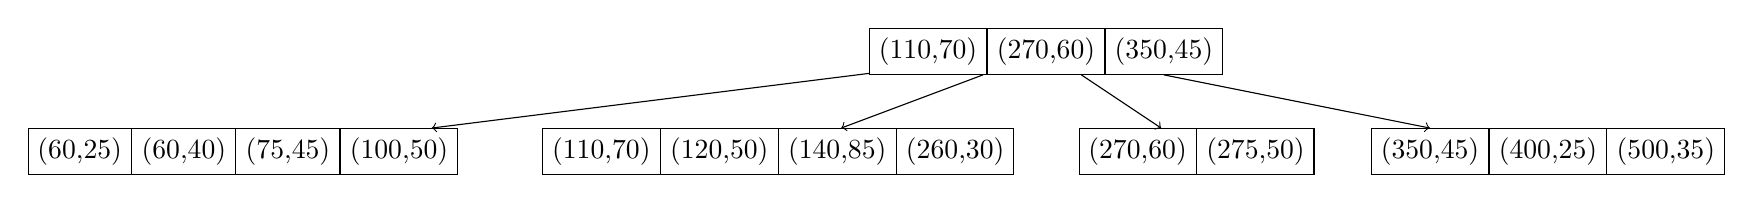
\begin{tikzpicture}[scale=.85]
  \tikzstyle{bplus}=[rectangle split, rectangle split horizontal,rectangle split ignore empty parts,draw]
  \tikzstyle{every node}=[bplus]
  \tikzstyle{level 1}=[sibling distance=80mm]
  \node {(110,70) \nodepart {two} (270,60) \nodepart{three} (350,45)} [->]
    child {node {(60,25) \nodepart{two} (60,40) \nodepart{three} (75,45) \nodepart{four} (100,50)}}
    child {node {(110,70) \nodepart{two} (120,50) \nodepart{three} (140,85) \nodepart{four} (260,30)}}
    child[sibling distance=45mm] {node {(270,60) \nodepart{two} (275,50)}}
    child[sibling distance=50mm] {node {(350,45) \nodepart{two} (400,25) \nodepart{three} (500,35)}}
  ;\end{tikzpicture}
  \end{small}
  \end{sideways}
  \end{center}
  \item \emph{Auf welche Schlüsselwerte des B\textsuperscript{+}-Baumes aus Nr. 2 muss nun zugegriffen werden, um die Queries aus Nr.1 mit dessen Hilfe zu beantworten?}
  \begin{enumerate}[{(}a{)}]
    \item \emph{\code{salary = 120}}\\
    $(110,70),(120,50),(140,85)^*$
    \item \emph{\code{age = 50}}\\
    $(110,70),(60,25),(60,40),(75,45),(100,50),$\\ $(120,50),(140,85),(260,30),(270,60),(275,50)$\\
    $(350,45),(400,25),(500,35)$
    \item \emph{\code{salary <= 300 AND age <= 40}}\\
    $(110,70),(60,25),(60,40),(75,45),(100,50),$\\ $(120,50),(140,85),(260,30),(270,60),(275,50)$\\
    $(350,45)^*$
  \end{enumerate}
  $*$ Markieren das Ende der Suche, da außerhalb des Prädikats
\subExEnd{}
%
\newpage 
%
\exercise{}
\lstinputlisting[firstline=7]{03.sql}
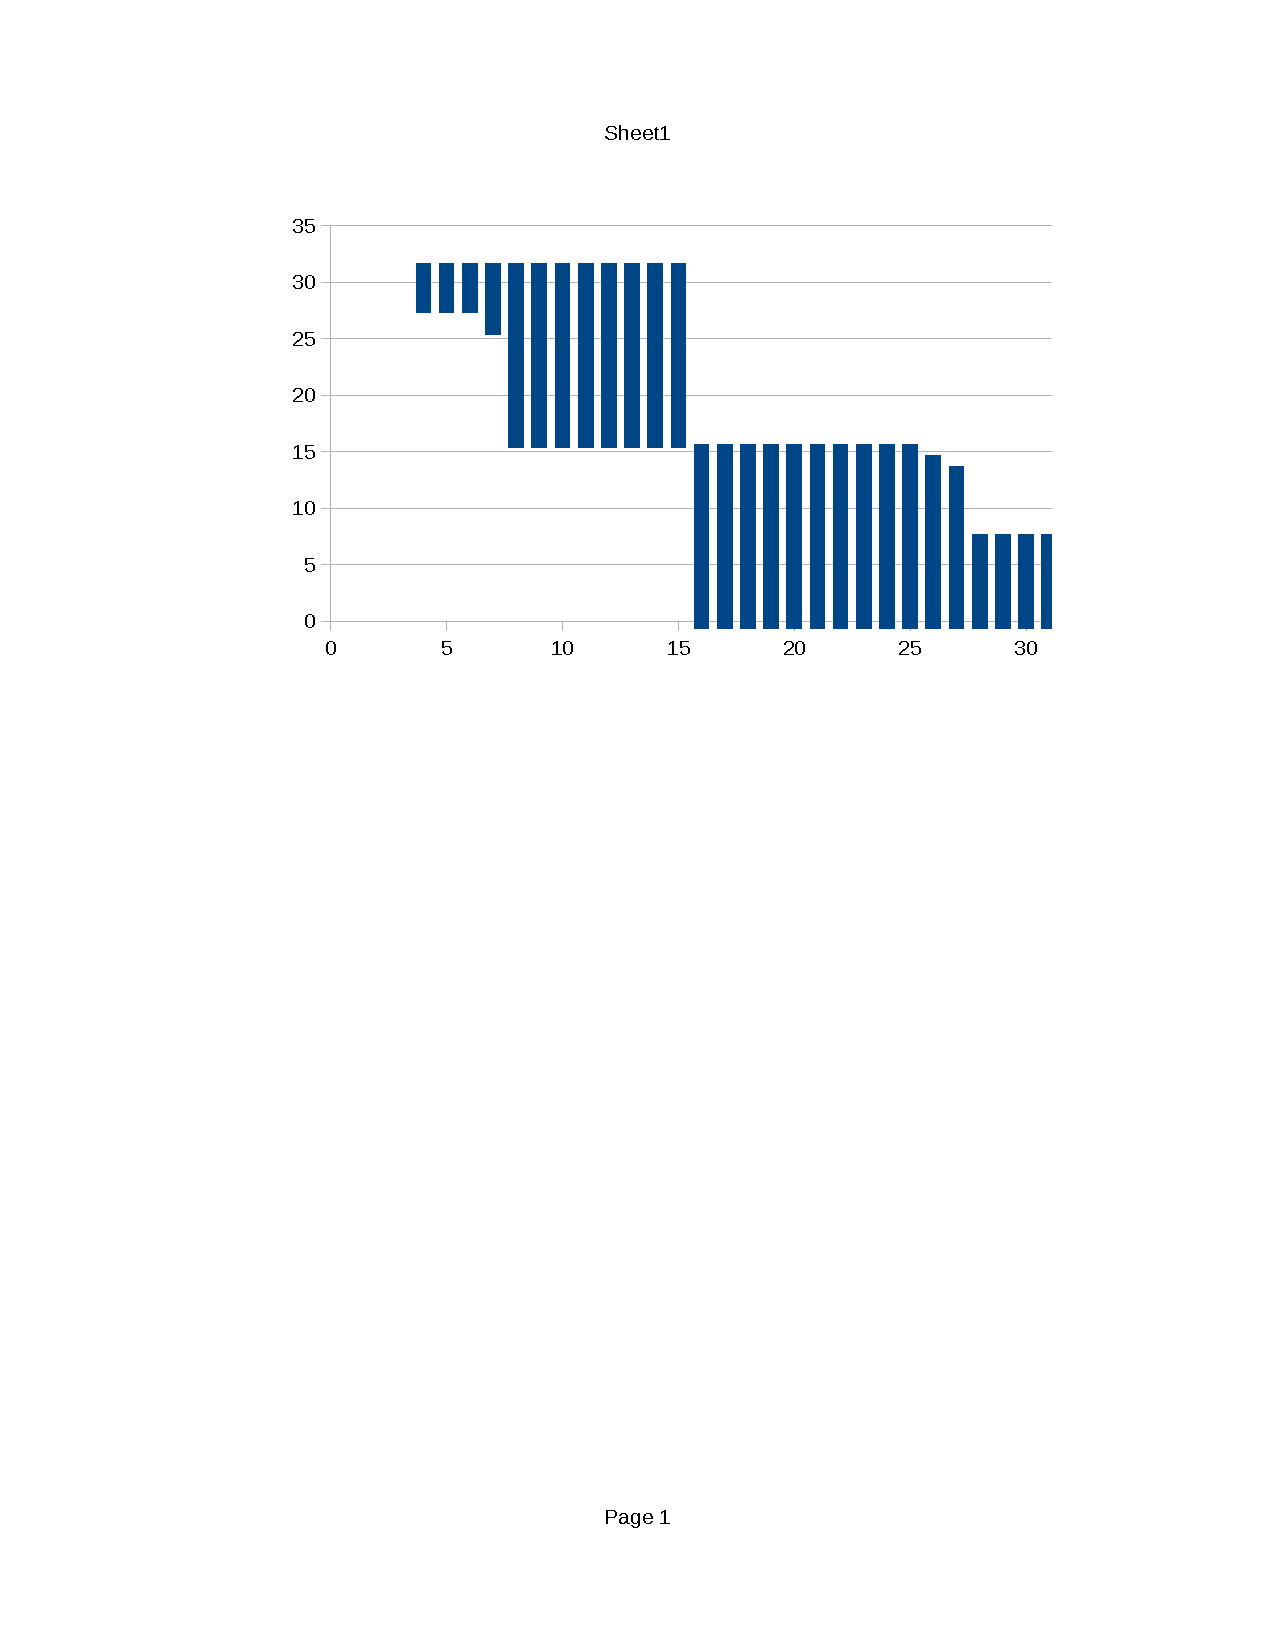
\includegraphics[]{./zindex.pdf}\\
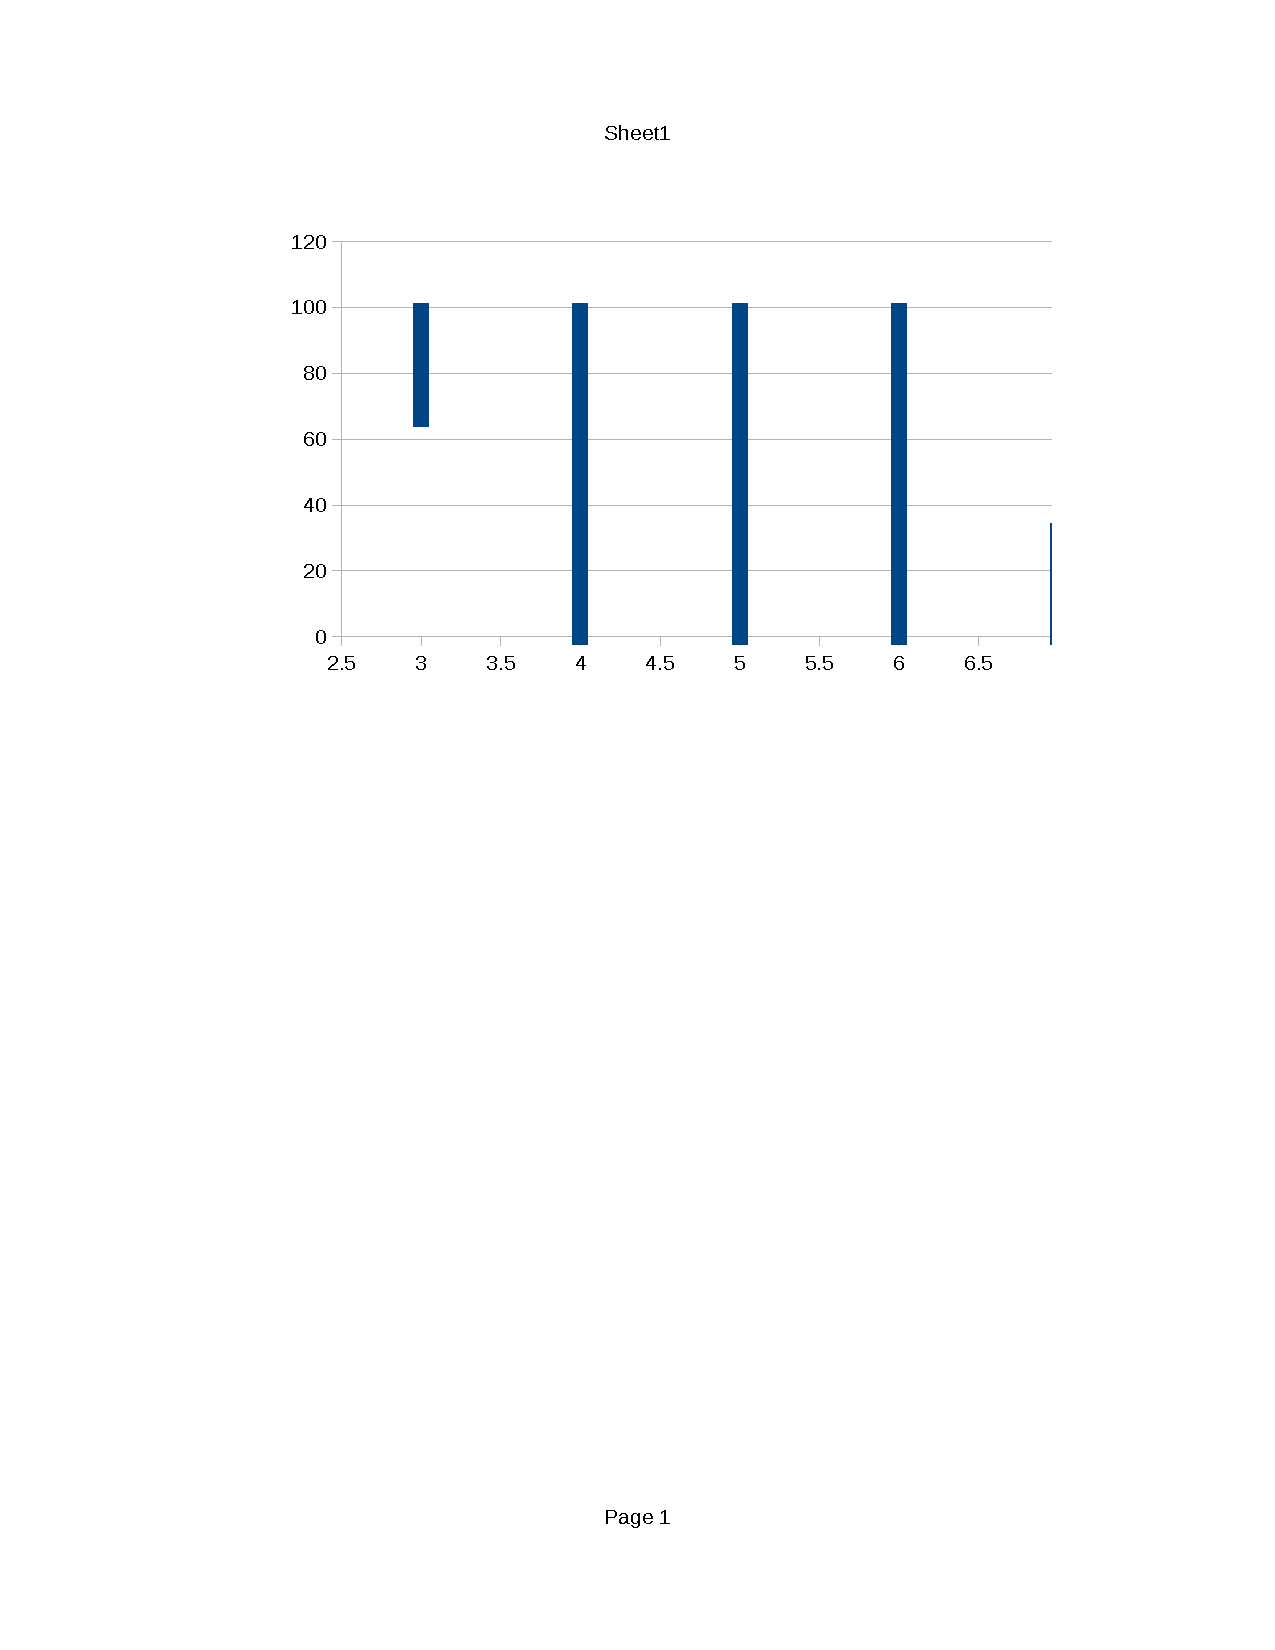
\includegraphics[]{./cindex.pdf}\\
Beim C-Index sind keine Zusammenhaenge ersichtlich.\\

Der Z-Index hingegen zeigt die Punkte auf einer in der Z Anordnung (verbindet man die Punkte zu einer Linie), da hier nach beiden Koordinaten sortiert wird.
\end{document}